% Options for packages loaded elsewhere
\PassOptionsToPackage{unicode}{hyperref}
\PassOptionsToPackage{hyphens}{url}
%
\documentclass[
]{article}
\usepackage{lmodern}
\usepackage{amssymb,amsmath}
\usepackage{ifxetex,ifluatex}
\ifnum 0\ifxetex 1\fi\ifluatex 1\fi=0 % if pdftex
  \usepackage[T1]{fontenc}
  \usepackage[utf8]{inputenc}
  \usepackage{textcomp} % provide euro and other symbols
\else % if luatex or xetex
  \usepackage{unicode-math}
  \defaultfontfeatures{Scale=MatchLowercase}
  \defaultfontfeatures[\rmfamily]{Ligatures=TeX,Scale=1}
\fi
% Use upquote if available, for straight quotes in verbatim environments
\IfFileExists{upquote.sty}{\usepackage{upquote}}{}
\IfFileExists{microtype.sty}{% use microtype if available
  \usepackage[]{microtype}
  \UseMicrotypeSet[protrusion]{basicmath} % disable protrusion for tt fonts
}{}
\makeatletter
\@ifundefined{KOMAClassName}{% if non-KOMA class
  \IfFileExists{parskip.sty}{%
    \usepackage{parskip}
  }{% else
    \setlength{\parindent}{0pt}
    \setlength{\parskip}{6pt plus 2pt minus 1pt}}
}{% if KOMA class
  \KOMAoptions{parskip=half}}
\makeatother
\usepackage{xcolor}
\IfFileExists{xurl.sty}{\usepackage{xurl}}{} % add URL line breaks if available
\IfFileExists{bookmark.sty}{\usepackage{bookmark}}{\usepackage{hyperref}}
\hypersetup{
  pdftitle={Analysis Using Natural Logarithm with Interaction Term},
  hidelinks,
  pdfcreator={LaTeX via pandoc}}
\urlstyle{same} % disable monospaced font for URLs
\usepackage[margin=1in]{geometry}
\usepackage{color}
\usepackage{fancyvrb}
\newcommand{\VerbBar}{|}
\newcommand{\VERB}{\Verb[commandchars=\\\{\}]}
\DefineVerbatimEnvironment{Highlighting}{Verbatim}{commandchars=\\\{\}}
% Add ',fontsize=\small' for more characters per line
\usepackage{framed}
\definecolor{shadecolor}{RGB}{248,248,248}
\newenvironment{Shaded}{\begin{snugshade}}{\end{snugshade}}
\newcommand{\AlertTok}[1]{\textcolor[rgb]{0.94,0.16,0.16}{#1}}
\newcommand{\AnnotationTok}[1]{\textcolor[rgb]{0.56,0.35,0.01}{\textbf{\textit{#1}}}}
\newcommand{\AttributeTok}[1]{\textcolor[rgb]{0.77,0.63,0.00}{#1}}
\newcommand{\BaseNTok}[1]{\textcolor[rgb]{0.00,0.00,0.81}{#1}}
\newcommand{\BuiltInTok}[1]{#1}
\newcommand{\CharTok}[1]{\textcolor[rgb]{0.31,0.60,0.02}{#1}}
\newcommand{\CommentTok}[1]{\textcolor[rgb]{0.56,0.35,0.01}{\textit{#1}}}
\newcommand{\CommentVarTok}[1]{\textcolor[rgb]{0.56,0.35,0.01}{\textbf{\textit{#1}}}}
\newcommand{\ConstantTok}[1]{\textcolor[rgb]{0.00,0.00,0.00}{#1}}
\newcommand{\ControlFlowTok}[1]{\textcolor[rgb]{0.13,0.29,0.53}{\textbf{#1}}}
\newcommand{\DataTypeTok}[1]{\textcolor[rgb]{0.13,0.29,0.53}{#1}}
\newcommand{\DecValTok}[1]{\textcolor[rgb]{0.00,0.00,0.81}{#1}}
\newcommand{\DocumentationTok}[1]{\textcolor[rgb]{0.56,0.35,0.01}{\textbf{\textit{#1}}}}
\newcommand{\ErrorTok}[1]{\textcolor[rgb]{0.64,0.00,0.00}{\textbf{#1}}}
\newcommand{\ExtensionTok}[1]{#1}
\newcommand{\FloatTok}[1]{\textcolor[rgb]{0.00,0.00,0.81}{#1}}
\newcommand{\FunctionTok}[1]{\textcolor[rgb]{0.00,0.00,0.00}{#1}}
\newcommand{\ImportTok}[1]{#1}
\newcommand{\InformationTok}[1]{\textcolor[rgb]{0.56,0.35,0.01}{\textbf{\textit{#1}}}}
\newcommand{\KeywordTok}[1]{\textcolor[rgb]{0.13,0.29,0.53}{\textbf{#1}}}
\newcommand{\NormalTok}[1]{#1}
\newcommand{\OperatorTok}[1]{\textcolor[rgb]{0.81,0.36,0.00}{\textbf{#1}}}
\newcommand{\OtherTok}[1]{\textcolor[rgb]{0.56,0.35,0.01}{#1}}
\newcommand{\PreprocessorTok}[1]{\textcolor[rgb]{0.56,0.35,0.01}{\textit{#1}}}
\newcommand{\RegionMarkerTok}[1]{#1}
\newcommand{\SpecialCharTok}[1]{\textcolor[rgb]{0.00,0.00,0.00}{#1}}
\newcommand{\SpecialStringTok}[1]{\textcolor[rgb]{0.31,0.60,0.02}{#1}}
\newcommand{\StringTok}[1]{\textcolor[rgb]{0.31,0.60,0.02}{#1}}
\newcommand{\VariableTok}[1]{\textcolor[rgb]{0.00,0.00,0.00}{#1}}
\newcommand{\VerbatimStringTok}[1]{\textcolor[rgb]{0.31,0.60,0.02}{#1}}
\newcommand{\WarningTok}[1]{\textcolor[rgb]{0.56,0.35,0.01}{\textbf{\textit{#1}}}}
\usepackage{graphicx,grffile}
\makeatletter
\def\maxwidth{\ifdim\Gin@nat@width>\linewidth\linewidth\else\Gin@nat@width\fi}
\def\maxheight{\ifdim\Gin@nat@height>\textheight\textheight\else\Gin@nat@height\fi}
\makeatother
% Scale images if necessary, so that they will not overflow the page
% margins by default, and it is still possible to overwrite the defaults
% using explicit options in \includegraphics[width, height, ...]{}
\setkeys{Gin}{width=\maxwidth,height=\maxheight,keepaspectratio}
% Set default figure placement to htbp
\makeatletter
\def\fps@figure{htbp}
\makeatother
\setlength{\emergencystretch}{3em} % prevent overfull lines
\providecommand{\tightlist}{%
  \setlength{\itemsep}{0pt}\setlength{\parskip}{0pt}}
\setcounter{secnumdepth}{-\maxdimen} % remove section numbering

\title{Analysis Using Natural Logarithm with Interaction Term}
\author{}
\date{\vspace{-2.5em}}

\begin{document}
\maketitle

\hypertarget{summary}{%
\section{Summary}\label{summary}}

Applying a modified linear regression model for better interpretability,
we found only a few changes in significance of relationship. Using the
model:
\[ln(R_j) = \alpha + \beta T_i + \gamma ln(t) + \sum_n \delta I_n + \sum_n \lambda_n I_n t\]
we found similar results for most of the regressions performed.

The main difference observed would be the reduced significance of all
training indices with the worker reallocation rate . The correlation
between worker reallocation rate and RL However, PT retains its strong
correlation. In general, most of the regressions have a lower R-squared
after the modification, but reamins high.

\hypertarget{naics-classification}{%
\section{NAICS Classification}\label{naics-classification}}

Due to the uneven nature of the datasets used, the industry classified
in the Business Employment Dynamics dataset (Job Reallocation Rate)
differs from the JOLTS dataset (Worker Reallocation Rate). The following
links would provide the mappings of the industry to the NAICS code.

\begin{itemize}
\tightlist
\item
  BED - \url{https://unl.box.com/s/dneof6j9qk8087fr5nvhi0vtn58mpcnw}
\item
  JOLTS - \url{https://unl.box.com/s/sgu028wja5eack5yqnbmt11lanc66bt5}
\end{itemize}

\hypertarget{job-reallocation-rate}{%
\section{Job Reallocation Rate}\label{job-reallocation-rate}}

Job Reallocation Rate refers to total jobs created plus total jobs
destroyed, divided by total jobs in the economy. This measure allows us
to look at how quickly jobs are reallocated from shrinking firms to
expanding ones.

The data source for job reallocation is from the Business Employment
Dynamics which collects quarterly job creation and destruction of firms.

Job Reallocation \textbf{does not} include workers switching jobs if the
job is not created or destroyed.

\hypertarget{results}{%
\subsection{Results}\label{results}}

\hypertarget{in-planton-site-training-pt}{%
\subsubsection{In-Plant/On-Site Training
(PT)}\label{in-planton-site-training-pt}}

\begin{Shaded}
\begin{Highlighting}[]
\NormalTok{lmod <-}\StringTok{ }\KeywordTok{lm}\NormalTok{(}\KeywordTok{log}\NormalTok{(adj_realloc) }\OperatorTok{~}\StringTok{  }\KeywordTok{log}\NormalTok{(PT) }\OperatorTok{+}\StringTok{ }\NormalTok{industryCategory}\OperatorTok{*}\NormalTok{period.num, t)}
\KeywordTok{summary}\NormalTok{(lmod)}
\end{Highlighting}
\end{Shaded}

\begin{verbatim}
## 
## Call:
## lm(formula = log(adj_realloc) ~ log(PT) + industryCategory * 
##     period.num, data = t)
## 
## Residuals:
##       Min        1Q    Median        3Q       Max 
## -0.169777 -0.020501  0.000132  0.020105  0.205155 
## 
## Coefficients:
##                                 Estimate Std. Error t value Pr(>|t|)    
## (Intercept)                    3.648e+00  5.178e-01   7.044 1.86e-11 ***
## log(PT)                        1.451e-01  4.704e-01   0.309 0.757940    
## industryCategory21            -1.388e+00  8.825e-02 -15.731  < 2e-16 ***
## industryCategory22            -2.230e+00  1.341e-01 -16.636  < 2e-16 ***
## industryCategory23            -6.524e-01  1.666e-01  -3.917 0.000116 ***
## industryCategory31            -1.653e+00  6.018e-02 -27.462  < 2e-16 ***
## industryCategory42            -1.399e+00  4.557e-02 -30.702  < 2e-16 ***
## industryCategory44            -1.175e+00  4.512e-02 -26.033  < 2e-16 ***
## industryCategory48            -1.366e+00  3.625e-02 -37.684  < 2e-16 ***
## industryCategory51            -1.547e+00  5.269e-02 -29.357  < 2e-16 ***
## industryCategory52            -1.503e+00  3.773e-02 -39.848  < 2e-16 ***
## industryCategory53            -1.064e+00  4.539e-02 -23.434  < 2e-16 ***
## industryCategory54            -1.105e+00  6.562e-02 -16.832  < 2e-16 ***
## industryCategory55            -1.821e+00  5.828e-02 -31.238  < 2e-16 ***
## industryCategory56            -8.233e-01  3.748e-02 -21.964  < 2e-16 ***
## industryCategory61            -1.208e+00  4.624e-02 -26.115  < 2e-16 ***
## industryCategory62            -1.663e+00  5.301e-02 -31.364  < 2e-16 ***
## industryCategory71            -4.029e-01  5.337e-02  -7.550 8.50e-13 ***
## industryCategory72            -9.715e-01  1.197e-01  -8.117 2.30e-14 ***
## industryCategory81            -1.047e+00  3.596e-02 -29.124  < 2e-16 ***
## period.num                    -1.681e-02  2.641e-03  -6.365 9.49e-10 ***
## industryCategory21:period.num  2.025e-02  3.742e-03   5.410 1.49e-07 ***
## industryCategory22:period.num  5.912e-03  3.746e-03   1.578 0.115749    
## industryCategory23:period.num  1.518e-03  3.735e-03   0.406 0.684754    
## industryCategory31:period.num -5.085e-03  3.728e-03  -1.364 0.173803    
## industryCategory42:period.num  9.516e-05  3.721e-03   0.026 0.979620    
## industryCategory44:period.num  2.424e-03  3.721e-03   0.651 0.515344    
## industryCategory48:period.num  1.015e-02  3.724e-03   2.725 0.006888 ** 
## industryCategory51:period.num  2.097e-02  3.756e-03   5.584 6.21e-08 ***
## industryCategory52:period.num -6.196e-03  3.792e-03  -1.634 0.103569    
## industryCategory53:period.num  3.050e-03  3.821e-03   0.798 0.425584    
## industryCategory54:period.num  2.015e-03  3.795e-03   0.531 0.596020    
## industryCategory55:period.num  3.240e-03  3.721e-03   0.871 0.384733    
## industryCategory56:period.num  4.095e-03  3.746e-03   1.093 0.275466    
## industryCategory61:period.num  1.179e-02  3.721e-03   3.170 0.001719 ** 
## industryCategory62:period.num  8.184e-03  4.099e-03   1.997 0.046960 *  
## industryCategory71:period.num  8.768e-03  3.730e-03   2.351 0.019526 *  
## industryCategory72:period.num  7.075e-03  3.762e-03   1.881 0.061204 .  
## industryCategory81:period.num  6.809e-03  3.722e-03   1.829 0.068576 .  
## ---
## Signif. codes:  0 '***' 0.001 '**' 0.01 '*' 0.05 '.' 0.1 ' ' 1
## 
## Residual standard error: 0.04403 on 246 degrees of freedom
## Multiple R-squared:  0.9933, Adjusted R-squared:  0.9923 
## F-statistic: 958.1 on 38 and 246 DF,  p-value: < 2.2e-16
\end{verbatim}

\hypertarget{on-the-job-training-oj}{%
\subsubsection{On-the-Job Training (OJ)}\label{on-the-job-training-oj}}

\begin{Shaded}
\begin{Highlighting}[]
\NormalTok{lmod <-}\StringTok{ }\KeywordTok{lm}\NormalTok{(}\KeywordTok{log}\NormalTok{(adj_realloc) }\OperatorTok{~}\StringTok{  }\KeywordTok{log}\NormalTok{(OJ) }\OperatorTok{+}\StringTok{ }\NormalTok{industryCategory}\OperatorTok{*}\NormalTok{period.num, t)}
\KeywordTok{summary}\NormalTok{(lmod)}
\end{Highlighting}
\end{Shaded}

\begin{verbatim}
## 
## Call:
## lm(formula = log(adj_realloc) ~ log(OJ) + industryCategory * 
##     period.num, data = t)
## 
## Residuals:
##       Min        1Q    Median        3Q       Max 
## -0.164257 -0.021699 -0.000515  0.020833  0.206381 
## 
## Coefficients:
##                                 Estimate Std. Error t value Pr(>|t|)    
## (Intercept)                    4.8961119  0.8517498   5.748 2.66e-08 ***
## log(OJ)                       -0.9182049  0.7180909  -1.279 0.202217    
## industryCategory21            -1.1726045  0.1527619  -7.676 3.85e-13 ***
## industryCategory22            -1.9039617  0.2263265  -8.412 3.31e-15 ***
## industryCategory23            -0.2850770  0.2501732  -1.140 0.255595    
## industryCategory31            -1.5170976  0.0998971 -15.187  < 2e-16 ***
## industryCategory42            -1.3411789  0.0507563 -26.424  < 2e-16 ***
## industryCategory44            -1.2312530  0.0501733 -24.540  < 2e-16 ***
## industryCategory48            -1.3560385  0.0340425 -39.834  < 2e-16 ***
## industryCategory51            -1.4512060  0.0732797 -19.804  < 2e-16 ***
## industryCategory52            -1.4280936  0.0643745 -22.184  < 2e-16 ***
## industryCategory53            -0.9582818  0.0824161 -11.627  < 2e-16 ***
## industryCategory54            -0.9203263  0.1348209  -6.826 6.76e-11 ***
## industryCategory55            -1.6885561  0.0978855 -17.250  < 2e-16 ***
## industryCategory56            -0.8629361  0.0432747 -19.941  < 2e-16 ***
## industryCategory61            -1.1421850  0.0551242 -20.720  < 2e-16 ***
## industryCategory62            -1.7178699  0.0474553 -36.200  < 2e-16 ***
## industryCategory71            -0.5060278  0.0783269  -6.460 5.55e-10 ***
## industryCategory72            -1.2430676  0.1877295  -6.622 2.21e-10 ***
## industryCategory81            -0.9821332  0.0586900 -16.734  < 2e-16 ***
## period.num                    -0.0166326  0.0026242  -6.338 1.10e-09 ***
## industryCategory21:period.num  0.0210505  0.0037797   5.569 6.69e-08 ***
## industryCategory22:period.num  0.0075070  0.0038816   1.934 0.054261 .  
## industryCategory23:period.num  0.0012596  0.0037114   0.339 0.734603    
## industryCategory31:period.num -0.0035461  0.0038833  -0.913 0.362048    
## industryCategory42:period.num  0.0009505  0.0037679   0.252 0.801053    
## industryCategory44:period.num  0.0026506  0.0037135   0.714 0.476045    
## industryCategory48:period.num  0.0094166  0.0037479   2.513 0.012628 *  
## industryCategory51:period.num  0.0237397  0.0043580   5.447 1.24e-07 ***
## industryCategory52:period.num -0.0032634  0.0042710  -0.764 0.445549    
## industryCategory53:period.num  0.0050507  0.0039493   1.279 0.202145    
## industryCategory54:period.num  0.0030746  0.0038443   0.800 0.424609    
## industryCategory55:period.num  0.0057551  0.0041933   1.372 0.171170    
## industryCategory56:period.num  0.0052637  0.0037967   1.386 0.166884    
## industryCategory61:period.num  0.0127563  0.0037846   3.371 0.000871 ***
## industryCategory62:period.num  0.0079515  0.0037570   2.116 0.035312 *  
## industryCategory71:period.num  0.0096220  0.0037587   2.560 0.011067 *  
## industryCategory72:period.num  0.0066793  0.0037136   1.799 0.073306 .  
## industryCategory81:period.num  0.0071049  0.0037182   1.911 0.057188 .  
## ---
## Signif. codes:  0 '***' 0.001 '**' 0.01 '*' 0.05 '.' 0.1 ' ' 1
## 
## Residual standard error: 0.04389 on 246 degrees of freedom
## Multiple R-squared:  0.9933, Adjusted R-squared:  0.9923 
## F-statistic: 964.1 on 38 and 246 DF,  p-value: < 2.2e-16
\end{verbatim}

\hypertarget{relevant-work-experience-rw}{%
\subsubsection{Relevant Work Experience
(RW)}\label{relevant-work-experience-rw}}

\begin{Shaded}
\begin{Highlighting}[]
\NormalTok{lmod <-}\StringTok{ }\KeywordTok{lm}\NormalTok{(}\KeywordTok{log}\NormalTok{(adj_realloc) }\OperatorTok{~}\StringTok{  }\KeywordTok{log}\NormalTok{(RW) }\OperatorTok{+}\StringTok{ }\NormalTok{industryCategory}\OperatorTok{*}\NormalTok{period.num, t)}
\KeywordTok{summary}\NormalTok{(lmod)}
\end{Highlighting}
\end{Shaded}

\begin{verbatim}
## 
## Call:
## lm(formula = log(adj_realloc) ~ log(RW) + industryCategory * 
##     period.num, data = t)
## 
## Residuals:
##       Min        1Q    Median        3Q       Max 
## -0.169340 -0.020129 -0.000139  0.020284  0.203781 
## 
## Coefficients:
##                                 Estimate Std. Error t value Pr(>|t|)    
## (Intercept)                    3.0868005  0.7726274   3.995 8.54e-05 ***
## log(RW)                        0.4970461  0.5326581   0.933  0.35166    
## industryCategory21            -1.4799228  0.1296517 -11.415  < 2e-16 ***
## industryCategory22            -2.3514048  0.1761011 -13.353  < 2e-16 ***
## industryCategory23            -0.7529313  0.1651854  -4.558 8.14e-06 ***
## industryCategory31            -1.7325112  0.1074447 -16.125  < 2e-16 ***
## industryCategory42            -1.5194359  0.1430965 -10.618  < 2e-16 ***
## industryCategory44            -1.1681981  0.0376683 -31.013  < 2e-16 ***
## industryCategory48            -1.3854427  0.0421237 -32.890  < 2e-16 ***
## industryCategory51            -1.6821213  0.1618760 -10.391  < 2e-16 ***
## industryCategory52            -1.6100249  0.1244996 -12.932  < 2e-16 ***
## industryCategory53            -1.1371628  0.0948696 -11.987  < 2e-16 ***
## industryCategory54            -1.2758989  0.2049810  -6.224 2.07e-09 ***
## industryCategory55            -1.9917235  0.2018171  -9.869  < 2e-16 ***
## industryCategory56            -0.8455770  0.0385382 -21.941  < 2e-16 ***
## industryCategory61            -1.2843469  0.0985675 -13.030  < 2e-16 ***
## industryCategory62            -1.6952985  0.0400717 -42.307  < 2e-16 ***
## industryCategory71            -0.4415791  0.0437504 -10.093  < 2e-16 ***
## industryCategory72            -0.9054405  0.1138837  -7.951 6.73e-14 ***
## industryCategory81            -1.1185597  0.0871925 -12.829  < 2e-16 ***
## period.num                    -0.0165933  0.0026316  -6.305 1.32e-09 ***
## industryCategory21:period.num  0.0189626  0.0039177   4.840 2.29e-06 ***
## industryCategory22:period.num  0.0047044  0.0039833   1.181  0.23872    
## industryCategory23:period.num  0.0007310  0.0037872   0.193  0.84710    
## industryCategory31:period.num -0.0062018  0.0039267  -1.579  0.11553    
## industryCategory42:period.num -0.0006620  0.0038049  -0.174  0.86203    
## industryCategory44:period.num  0.0022263  0.0037213   0.598  0.55023    
## industryCategory48:period.num  0.0097247  0.0037370   2.602  0.00982 ** 
## industryCategory51:period.num  0.0188962  0.0042462   4.450 1.30e-05 ***
## industryCategory52:period.num -0.0072632  0.0039651  -1.832  0.06819 .  
## industryCategory53:period.num  0.0023613  0.0038539   0.613  0.54063    
## industryCategory54:period.num  0.0003081  0.0040378   0.076  0.93924    
## industryCategory55:period.num  0.0009187  0.0044799   0.205  0.83769    
## industryCategory56:period.num  0.0032094  0.0038723   0.829  0.40802    
## industryCategory61:period.num  0.0109148  0.0038334   2.847  0.00478 ** 
## industryCategory62:period.num  0.0070439  0.0041238   1.708  0.08888 .  
## industryCategory71:period.num  0.0083377  0.0037549   2.220  0.02730 *  
## industryCategory72:period.num  0.0066544  0.0037248   1.787  0.07524 .  
## industryCategory81:period.num  0.0061045  0.0037846   1.613  0.10804    
## ---
## Signif. codes:  0 '***' 0.001 '**' 0.01 '*' 0.05 '.' 0.1 ' ' 1
## 
## Residual standard error: 0.04396 on 246 degrees of freedom
## Multiple R-squared:  0.9933, Adjusted R-squared:  0.9923 
## F-statistic: 961.1 on 38 and 246 DF,  p-value: < 2.2e-16
\end{verbatim}

\hypertarget{required-level-of-education-rl}{%
\subsubsection{Required Level of Education
(RL)}\label{required-level-of-education-rl}}

\begin{Shaded}
\begin{Highlighting}[]
\NormalTok{lmod <-}\StringTok{ }\KeywordTok{lm}\NormalTok{(}\KeywordTok{log}\NormalTok{(adj_realloc) }\OperatorTok{~}\StringTok{  }\KeywordTok{log}\NormalTok{(RL) }\OperatorTok{+}\StringTok{ }\NormalTok{industryCategory}\OperatorTok{*}\NormalTok{period.num, t)}
\KeywordTok{summary}\NormalTok{(lmod)}
\end{Highlighting}
\end{Shaded}

\begin{verbatim}
## 
## Call:
## lm(formula = log(adj_realloc) ~ log(RL) + industryCategory * 
##     period.num, data = t)
## 
## Residuals:
##       Min        1Q    Median        3Q       Max 
## -0.154593 -0.021187  0.001822  0.019200  0.190125 
## 
## Coefficients:
##                                 Estimate Std. Error t value Pr(>|t|)    
## (Intercept)                    2.7165945  0.2490616  10.907  < 2e-16 ***
## log(RL)                        1.1002307  0.2501303   4.399 1.62e-05 ***
## industryCategory21            -1.4895799  0.0434526 -34.281  < 2e-16 ***
## industryCategory22            -2.5377006  0.0854717 -29.691  < 2e-16 ***
## industryCategory23            -0.6088221  0.0326176 -18.665  < 2e-16 ***
## industryCategory31            -1.8054963  0.0502307 -35.944  < 2e-16 ***
## industryCategory42            -1.7223212  0.0823438 -20.916  < 2e-16 ***
## industryCategory44            -1.1337220  0.0345096 -32.852  < 2e-16 ***
## industryCategory48            -1.3742829  0.0327015 -42.025  < 2e-16 ***
## industryCategory51            -2.1003731  0.1327328 -15.824  < 2e-16 ***
## industryCategory52            -1.9729539  0.1127412 -17.500  < 2e-16 ***
## industryCategory53            -1.3048286  0.0655894 -19.894  < 2e-16 ***
## industryCategory54            -1.8879310  0.1849253 -10.209  < 2e-16 ***
## industryCategory55            -2.4492139  0.1498038 -16.349  < 2e-16 ***
## industryCategory56            -0.9662729  0.0452321 -21.363  < 2e-16 ***
## industryCategory61            -1.9897026  0.1829272 -10.877  < 2e-16 ***
## industryCategory62            -2.3280893  0.1519680 -15.320  < 2e-16 ***
## industryCategory71            -0.5574674  0.0458397 -12.161  < 2e-16 ***
## industryCategory72            -0.7533193  0.0662253 -11.375  < 2e-16 ***
## industryCategory81            -1.2429285  0.0558221 -22.266  < 2e-16 ***
## period.num                    -0.0193620  0.0026031  -7.438 1.70e-12 ***
## industryCategory21:period.num  0.0201127  0.0035835   5.613 5.36e-08 ***
## industryCategory22:period.num  0.0061929  0.0035836   1.728 0.085223 .  
## industryCategory23:period.num  0.0003136  0.0035922   0.087 0.930504    
## industryCategory31:period.num -0.0034000  0.0036022  -0.944 0.346161    
## industryCategory42:period.num  0.0021637  0.0036139   0.599 0.549912    
## industryCategory44:period.num  0.0044346  0.0036124   1.228 0.220769    
## industryCategory48:period.num  0.0140533  0.0036944   3.804 0.000180 ***
## industryCategory51:period.num  0.0240145  0.0036565   6.568 3.02e-10 ***
## industryCategory52:period.num -0.0058540  0.0035836  -1.634 0.103625    
## industryCategory53:period.num  0.0048889  0.0036012   1.358 0.175844    
## industryCategory54:period.num  0.0075514  0.0038158   1.979 0.048933 *  
## industryCategory55:period.num  0.0045260  0.0035951   1.259 0.209242    
## industryCategory56:period.num  0.0085074  0.0037131   2.291 0.022801 *  
## industryCategory61:period.num  0.0132135  0.0035979   3.673 0.000295 ***
## industryCategory62:period.num  0.0211859  0.0045695   4.636 5.76e-06 ***
## industryCategory71:period.num  0.0092174  0.0035844   2.572 0.010714 *  
## industryCategory72:period.num  0.0097471  0.0036413   2.677 0.007932 ** 
## industryCategory81:period.num  0.0076467  0.0035889   2.131 0.034109 *  
## ---
## Signif. codes:  0 '***' 0.001 '**' 0.01 '*' 0.05 '.' 0.1 ' ' 1
## 
## Residual standard error: 0.0424 on 246 degrees of freedom
## Multiple R-squared:  0.9938, Adjusted R-squared:  0.9928 
## F-statistic:  1034 on 38 and 246 DF,  p-value: < 2.2e-16
\end{verbatim}

\hypertarget{interpretation}{%
\subsection{Interpretation}\label{interpretation}}

As the result above shows, across industries and adjusted with time, PT,
OJ and RW are not statistically significant indices to explain the drop
in job reallocation rate. Nevertheless, the correlation between RL and
job reallocation rate is positive and statistically significant. This
suggests that a higher level of education could have a positive
influence job reallocation within industry.

Most previous literature found that training indices and reallocation
rate have a negative relationship. This is true for the economy as a
whole as shown in the graph below. Without including the interaction
term between time and industry, there is a statistically significant
negative relationship with the training indices.

\begin{Shaded}
\begin{Highlighting}[]
\KeywordTok{ggplot}\NormalTok{(}\DataTypeTok{data =}\NormalTok{ t) }\OperatorTok{+}
\StringTok{  }\KeywordTok{geom_point}\NormalTok{(}\DataTypeTok{mapping =} \KeywordTok{aes}\NormalTok{(RW, adj_realloc, }\DataTypeTok{colour =}\NormalTok{ NAICS)) }\OperatorTok{+}
\StringTok{  }\KeywordTok{xlab}\NormalTok{(}\StringTok{'Required Level of Education'}\NormalTok{) }\OperatorTok{+}\StringTok{ }
\StringTok{  }\KeywordTok{ylab}\NormalTok{(}\StringTok{'Job Reallocation Rate'}\NormalTok{) }\OperatorTok{+}\StringTok{ }
\StringTok{  }\KeywordTok{ggtitle}\NormalTok{(}\StringTok{"Required Level of Education and Job Reallocation Rate"}\NormalTok{) }\OperatorTok{+}
\StringTok{  }\KeywordTok{theme_light}\NormalTok{()}
\end{Highlighting}
\end{Shaded}

\begin{figure}
\centering
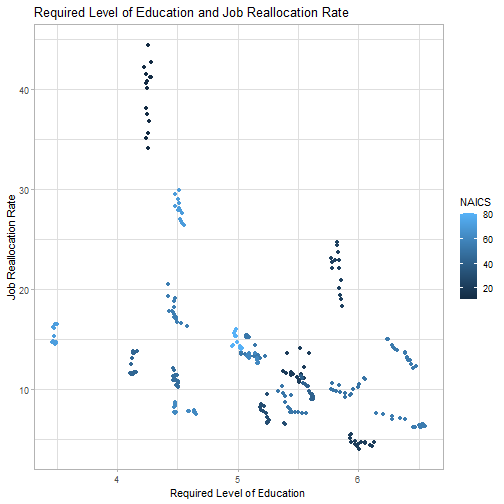
\includegraphics{figure/unnamed-chunk-6-1.png}
\caption{plot of chunk unnamed-chunk-6}
\end{figure}

However, when dummies are included, the relationship holds for some but
not for all. In the previous analysis, with only dummy variables for
industry categories, RW, OJ and PT have statistically significant
negative relationship with job reallocation rate (only RL has an
insignificant relationship). Nevertheless, with the addition of the
interaction term between industry category and time, RW, OJ and PT has
become insignificant explanations for the declining job reallocation
rate while RL becomes significant in describing it with a
\textbf{positive relationship}!

Since the \(R^2\) value increased and all of the interactive terms are
statistically significant, it is likely that idiosyncracies in the
labour market of specific industry as well as another variable that is
changing across time could better explain the trend of declining job
reallocation rate across time.

\begin{Shaded}
\begin{Highlighting}[]
\NormalTok{lmod <-}\StringTok{ }\KeywordTok{lm}\NormalTok{(}\KeywordTok{log}\NormalTok{(adj_realloc) }\OperatorTok{~}\StringTok{ }\KeywordTok{log}\NormalTok{(RL) }\OperatorTok{+}\StringTok{ }\NormalTok{industryCategory}\OperatorTok{*}\NormalTok{period.num, t)}
\KeywordTok{summary}\NormalTok{(lmod)}
\end{Highlighting}
\end{Shaded}

\begin{verbatim}
## 
## Call:
## lm(formula = log(adj_realloc) ~ log(RL) + industryCategory * 
##     period.num, data = t)
## 
## Residuals:
##       Min        1Q    Median        3Q       Max 
## -0.154593 -0.021187  0.001822  0.019200  0.190125 
## 
## Coefficients:
##                                 Estimate Std. Error t value Pr(>|t|)    
## (Intercept)                    2.7165945  0.2490616  10.907  < 2e-16 ***
## log(RL)                        1.1002307  0.2501303   4.399 1.62e-05 ***
## industryCategory21            -1.4895799  0.0434526 -34.281  < 2e-16 ***
## industryCategory22            -2.5377006  0.0854717 -29.691  < 2e-16 ***
## industryCategory23            -0.6088221  0.0326176 -18.665  < 2e-16 ***
## industryCategory31            -1.8054963  0.0502307 -35.944  < 2e-16 ***
## industryCategory42            -1.7223212  0.0823438 -20.916  < 2e-16 ***
## industryCategory44            -1.1337220  0.0345096 -32.852  < 2e-16 ***
## industryCategory48            -1.3742829  0.0327015 -42.025  < 2e-16 ***
## industryCategory51            -2.1003731  0.1327328 -15.824  < 2e-16 ***
## industryCategory52            -1.9729539  0.1127412 -17.500  < 2e-16 ***
## industryCategory53            -1.3048286  0.0655894 -19.894  < 2e-16 ***
## industryCategory54            -1.8879310  0.1849253 -10.209  < 2e-16 ***
## industryCategory55            -2.4492139  0.1498038 -16.349  < 2e-16 ***
## industryCategory56            -0.9662729  0.0452321 -21.363  < 2e-16 ***
## industryCategory61            -1.9897026  0.1829272 -10.877  < 2e-16 ***
## industryCategory62            -2.3280893  0.1519680 -15.320  < 2e-16 ***
## industryCategory71            -0.5574674  0.0458397 -12.161  < 2e-16 ***
## industryCategory72            -0.7533193  0.0662253 -11.375  < 2e-16 ***
## industryCategory81            -1.2429285  0.0558221 -22.266  < 2e-16 ***
## period.num                    -0.0193620  0.0026031  -7.438 1.70e-12 ***
## industryCategory21:period.num  0.0201127  0.0035835   5.613 5.36e-08 ***
## industryCategory22:period.num  0.0061929  0.0035836   1.728 0.085223 .  
## industryCategory23:period.num  0.0003136  0.0035922   0.087 0.930504    
## industryCategory31:period.num -0.0034000  0.0036022  -0.944 0.346161    
## industryCategory42:period.num  0.0021637  0.0036139   0.599 0.549912    
## industryCategory44:period.num  0.0044346  0.0036124   1.228 0.220769    
## industryCategory48:period.num  0.0140533  0.0036944   3.804 0.000180 ***
## industryCategory51:period.num  0.0240145  0.0036565   6.568 3.02e-10 ***
## industryCategory52:period.num -0.0058540  0.0035836  -1.634 0.103625    
## industryCategory53:period.num  0.0048889  0.0036012   1.358 0.175844    
## industryCategory54:period.num  0.0075514  0.0038158   1.979 0.048933 *  
## industryCategory55:period.num  0.0045260  0.0035951   1.259 0.209242    
## industryCategory56:period.num  0.0085074  0.0037131   2.291 0.022801 *  
## industryCategory61:period.num  0.0132135  0.0035979   3.673 0.000295 ***
## industryCategory62:period.num  0.0211859  0.0045695   4.636 5.76e-06 ***
## industryCategory71:period.num  0.0092174  0.0035844   2.572 0.010714 *  
## industryCategory72:period.num  0.0097471  0.0036413   2.677 0.007932 ** 
## industryCategory81:period.num  0.0076467  0.0035889   2.131 0.034109 *  
## ---
## Signif. codes:  0 '***' 0.001 '**' 0.01 '*' 0.05 '.' 0.1 ' ' 1
## 
## Residual standard error: 0.0424 on 246 degrees of freedom
## Multiple R-squared:  0.9938, Adjusted R-squared:  0.9928 
## F-statistic:  1034 on 38 and 246 DF,  p-value: < 2.2e-16
\end{verbatim}

\hypertarget{theoretical-explanations}{%
\subsection{Theoretical Explanations}\label{theoretical-explanations}}

A possible explanation of this phenomenon could come from the fact that
employers have little to no incentive in keeping jobs with high level of
educational requirement since investment in education is largely done by
the employee, not the employer. Hence, the costs of readjusting
employment if a mismatch occurs is lower, causing employers to be more
willing to fire employees with higher levels education.

It is also possible that mismatch occurs more frequently, given the
existence of asymmetric information for general training. Having a
degree proves that you could have the relevant skills to do the job but
it might turn out to be unsuitable for you.

Nevertheless, these explanations are also applicable to other training
indices but there is no statistically significant relationship between
them.

Using the formula
\(Job\ Reallocation = Job\ Creation + Job\ Destruction\), we can
decompose job reallocation rates to job creation rates and job
destruction rates. The following are the results on performing the
regressions using the formula below:

\[R_{job \ creation} = \alpha + \beta T_{RL} + \gamma t + \sum_n \delta I_n + \sum_n \lambda_n I_n t\]

\begin{Shaded}
\begin{Highlighting}[]
\NormalTok{lmod <-}\StringTok{ }\KeywordTok{lm}\NormalTok{(}\KeywordTok{log}\NormalTok{(gain) }\OperatorTok{~}\StringTok{ }\KeywordTok{log}\NormalTok{(RL) }\OperatorTok{+}\StringTok{ }\NormalTok{industryCategory}\OperatorTok{*}\NormalTok{period.num, t)}
\KeywordTok{summary}\NormalTok{(lmod)}
\end{Highlighting}
\end{Shaded}

\begin{verbatim}
## 
## Call:
## lm(formula = log(gain) ~ log(RL) + industryCategory * period.num, 
##     data = t)
## 
## Residuals:
##      Min       1Q   Median       3Q      Max 
## -0.39755 -0.02720  0.00794  0.03221  0.24473 
## 
## Coefficients:
##                                 Estimate Std. Error t value Pr(>|t|)    
## (Intercept)                    3.5143920  0.3900414   9.010  < 2e-16 ***
## log(RL)                       -0.4058578  0.3917150  -1.036 0.301171    
## industryCategory21            -1.1616597  0.0680486 -17.071  < 2e-16 ***
## industryCategory22            -2.0540542  0.1338525 -15.346  < 2e-16 ***
## industryCategory23            -0.6362762  0.0510806 -12.456  < 2e-16 ***
## industryCategory31            -1.6827559  0.0786635 -21.392  < 2e-16 ***
## industryCategory42            -1.2633446  0.1289540  -9.797  < 2e-16 ***
## industryCategory44            -1.1944442  0.0540436 -22.101  < 2e-16 ***
## industryCategory48            -1.3842844  0.0512120 -27.030  < 2e-16 ***
## industryCategory51            -1.3680508  0.2078653  -6.581 2.79e-10 ***
## industryCategory52            -1.3410985  0.1765576  -7.596 6.37e-13 ***
## industryCategory53            -0.9746014  0.1027159  -9.488  < 2e-16 ***
## industryCategory54            -0.7519749  0.2896011  -2.597 0.009982 ** 
## industryCategory55            -1.5861985  0.2345993  -6.761 9.88e-11 ***
## industryCategory56            -0.7648403  0.0708355 -10.797  < 2e-16 ***
## industryCategory61            -0.8393560  0.2864721  -2.930 0.003709 ** 
## industryCategory62            -1.3645553  0.2379886  -5.734 2.87e-08 ***
## industryCategory71            -0.3661174  0.0717870  -5.100 6.78e-07 ***
## industryCategory72            -1.0850164  0.1037117 -10.462  < 2e-16 ***
## industryCategory81            -0.9696034  0.0874198 -11.091  < 2e-16 ***
## period.num                    -0.0153631  0.0040766  -3.769 0.000206 ***
## industryCategory21:period.num  0.0048366  0.0056119   0.862 0.389605    
## industryCategory22:period.num  0.0036589  0.0056121   0.652 0.515037    
## industryCategory23:period.num  0.0066819  0.0056256   1.188 0.236071    
## industryCategory31:period.num  0.0043184  0.0056412   0.766 0.444701    
## industryCategory42:period.num  0.0012658  0.0056595   0.224 0.823208    
## industryCategory44:period.num  0.0011066  0.0056572   0.196 0.845079    
## industryCategory48:period.num  0.0154373  0.0057855   2.668 0.008131 ** 
## industryCategory51:period.num  0.0225842  0.0057263   3.944 0.000105 ***
## industryCategory52:period.num -0.0032590  0.0056120  -0.581 0.561961    
## industryCategory53:period.num  0.0057394  0.0056397   1.018 0.309825    
## industryCategory54:period.num -0.0001858  0.0059757  -0.031 0.975222    
## industryCategory55:period.num  0.0070966  0.0056301   1.260 0.208688    
## industryCategory56:period.num  0.0034641  0.0058149   0.596 0.551908    
## industryCategory61:period.num  0.0085319  0.0056345   1.514 0.131253    
## industryCategory62:period.num  0.0036216  0.0071561   0.506 0.613252    
## industryCategory71:period.num  0.0100029  0.0056134   1.782 0.075988 .  
## industryCategory72:period.num  0.0068622  0.0057024   1.203 0.229985    
## industryCategory81:period.num  0.0078415  0.0056204   1.395 0.164216    
## ---
## Signif. codes:  0 '***' 0.001 '**' 0.01 '*' 0.05 '.' 0.1 ' ' 1
## 
## Residual standard error: 0.0664 on 246 degrees of freedom
## Multiple R-squared:  0.9849, Adjusted R-squared:  0.9826 
## F-statistic:   422 on 38 and 246 DF,  p-value: < 2.2e-16
\end{verbatim}

\[R_{job \ destruction} = \alpha + \beta T_{RL} + \gamma t + \sum_n \delta I_n + \sum_n \lambda_n I_n t\]

\begin{Shaded}
\begin{Highlighting}[]
\NormalTok{lmod <-}\StringTok{ }\KeywordTok{lm}\NormalTok{(}\KeywordTok{log}\NormalTok{(loss) }\OperatorTok{~}\StringTok{ }\KeywordTok{log}\NormalTok{(RL) }\OperatorTok{+}\StringTok{ }\NormalTok{industryCategory}\OperatorTok{*}\NormalTok{period.num, t)}
\KeywordTok{summary}\NormalTok{(lmod)}
\end{Highlighting}
\end{Shaded}

\begin{verbatim}
## 
## Call:
## lm(formula = log(loss) ~ log(RL) + industryCategory * period.num, 
##     data = t)
## 
## Residuals:
##      Min       1Q   Median       3Q      Max 
## -0.28805 -0.03654 -0.00711  0.02862  0.56057 
## 
## Coefficients:
##                                Estimate Std. Error t value Pr(>|t|)    
## (Intercept)                    0.618428   0.522792   1.183 0.237978    
## log(RL)                        2.519515   0.525035   4.799 2.77e-06 ***
## industryCategory21            -1.834309   0.091209 -20.111  < 2e-16 ***
## industryCategory22            -2.997368   0.179409 -16.707  < 2e-16 ***
## industryCategory23            -0.588070   0.068466  -8.589 1.02e-15 ***
## industryCategory31            -1.933842   0.105437 -18.341  < 2e-16 ***
## industryCategory42            -2.160102   0.172843 -12.497  < 2e-16 ***
## industryCategory44            -1.079569   0.072437 -14.903  < 2e-16 ***
## industryCategory48            -1.366861   0.068642 -19.913  < 2e-16 ***
## industryCategory51            -2.792642   0.278612 -10.023  < 2e-16 ***
## industryCategory52            -2.571268   0.236649 -10.865  < 2e-16 ***
## industryCategory53            -1.617716   0.137675 -11.750  < 2e-16 ***
## industryCategory54            -2.964937   0.388167  -7.638 4.88e-13 ***
## industryCategory55            -3.265150   0.314445 -10.384  < 2e-16 ***
## industryCategory56            -1.161537   0.094944 -12.234  < 2e-16 ***
## industryCategory61            -3.081957   0.383973  -8.026 4.13e-14 ***
## industryCategory62            -3.245060   0.318988 -10.173  < 2e-16 ***
## industryCategory71            -0.737902   0.096220  -7.669 4.03e-13 ***
## industryCategory72            -0.442942   0.139010  -3.186 0.001627 ** 
## industryCategory81            -1.500982   0.117173 -12.810  < 2e-16 ***
## period.num                    -0.023152   0.005464  -4.237 3.20e-05 ***
## industryCategory21:period.num  0.032917   0.007522   4.376 1.79e-05 ***
## industryCategory22:period.num  0.008883   0.007522   1.181 0.238797    
## industryCategory23:period.num -0.005649   0.007540  -0.749 0.454443    
## industryCategory31:period.num -0.010225   0.007561  -1.352 0.177542    
## industryCategory42:period.num  0.003095   0.007586   0.408 0.683613    
## industryCategory44:period.num  0.007743   0.007583   1.021 0.308192    
## industryCategory48:period.num  0.012088   0.007755   1.559 0.120317    
## industryCategory51:period.num  0.025461   0.007675   3.317 0.001046 ** 
## industryCategory52:period.num -0.008268   0.007522  -1.099 0.272781    
## industryCategory53:period.num  0.003967   0.007559   0.525 0.600218    
## industryCategory54:period.num  0.014956   0.008010   1.867 0.063058 .  
## industryCategory55:period.num  0.001885   0.007546   0.250 0.802987    
## industryCategory56:period.num  0.013454   0.007794   1.726 0.085571 .  
## industryCategory61:period.num  0.018017   0.007552   2.386 0.017805 *  
## industryCategory62:period.num  0.037782   0.009592   3.939 0.000107 ***
## industryCategory71:period.num  0.008391   0.007524   1.115 0.265826    
## industryCategory72:period.num  0.012400   0.007643   1.622 0.106016    
## industryCategory81:period.num  0.007373   0.007533   0.979 0.328685    
## ---
## Signif. codes:  0 '***' 0.001 '**' 0.01 '*' 0.05 '.' 0.1 ' ' 1
## 
## Residual standard error: 0.089 on 246 degrees of freedom
## Multiple R-squared:  0.9735, Adjusted R-squared:  0.9694 
## F-statistic: 237.6 on 38 and 246 DF,  p-value: < 2.2e-16
\end{verbatim}

The results show that the main factor behind the positive relationship
observed between RL and job reallocation rate is job destruction rate
and not job creation rate. This is a little baffling given the general
consensus in empirical evidences that the US workforce as a whole is
increasingly educated and that employers are looking for highly educated
employees.

Nevertheless, most studies look at the labour market as a whole whilst
this does not take into account the compositional shift of industries in
the economy, only the required level of education of jobs within
industries.

\hypertarget{worker-reallocation-rate}{%
\section{Worker Reallocation Rate}\label{worker-reallocation-rate}}

Worker Reallocation refers to the sum of job finding and separations, it
is a common measure of labour market fluidity because it tracks not only
the creation and destruction of jobs, but also the flow of workers
unexplained by job creation and destruction.

Worker reallocation rate is defined as worker reallocation divided by
the labour force. The data is collected from JOLTS (Job Openings and
Labour Turnover Surveys), which has monthly data on job finding and
separations.

For separations, JOLTS categorize them into layoffs and discharges,
quits and other separations. This could help us further identify the
patterns within the labor market.

\hypertarget{results-1}{%
\subsection{Results}\label{results-1}}

\hypertarget{in-planton-site-training-pt-1}{%
\subsubsection{In-Plant/On-Site Training
(PT)}\label{in-planton-site-training-pt-1}}

\begin{Shaded}
\begin{Highlighting}[]
\NormalTok{lmod <-}\StringTok{ }\KeywordTok{lm}\NormalTok{(}\KeywordTok{log}\NormalTok{(realloc_rate) }\OperatorTok{~}\StringTok{ }\KeywordTok{log}\NormalTok{(PT) }\OperatorTok{+}\StringTok{ }\NormalTok{industryCategoryWR}\OperatorTok{*}\NormalTok{period.num, p)}
\KeywordTok{summary}\NormalTok{(lmod)}
\end{Highlighting}
\end{Shaded}

\begin{verbatim}
## 
## Call:
## lm(formula = log(realloc_rate) ~ log(PT) + industryCategoryWR * 
##     period.num, data = p)
## 
## Residuals:
##      Min       1Q   Median       3Q      Max 
## -0.22774 -0.05372  0.01082  0.05727  0.19437 
## 
## Coefficients:
##                                  Estimate Std. Error t value Pr(>|t|)    
## (Intercept)                     -0.464942   1.299119  -0.358 0.720815    
## log(PT)                          3.776399   1.019807   3.703 0.000278 ***
## industryCategoryWR23             0.056073   0.190305   0.295 0.768579    
## industryCategoryWR31             0.048341   0.098351   0.492 0.623615    
## industryCategoryWR42             0.259611   0.130970   1.982 0.048867 *  
## industryCategoryWR44             1.314456   0.251442   5.228 4.42e-07 ***
## industryCategoryWR48             0.522677   0.164284   3.182 0.001706 ** 
## industryCategoryWR51             0.086791   0.113506   0.765 0.445415    
## industryCategoryWR52             0.227917   0.157106   1.451 0.148472    
## industryCategoryWR53             0.655694   0.131455   4.988 1.35e-06 ***
## industryCategoryWR54             0.664927   0.089121   7.461 2.81e-12 ***
## industryCategoryWR61             0.144391   0.129152   1.118 0.264955    
## industryCategoryWR62             0.811014   0.274336   2.956 0.003500 ** 
## industryCategoryWR71             1.725998   0.275302   6.269 2.30e-09 ***
## industryCategoryWR72             2.257011   0.431371   5.232 4.33e-07 ***
## industryCategoryWR81             0.662836   0.165905   3.995 9.17e-05 ***
## period.num                       0.017837   0.005479   3.256 0.001335 ** 
## industryCategoryWR23:period.num -0.035302   0.007731  -4.566 8.81e-06 ***
## industryCategoryWR31:period.num -0.031708   0.007848  -4.040 7.69e-05 ***
## industryCategoryWR42:period.num -0.034535   0.007786  -4.436 1.54e-05 ***
## industryCategoryWR44:period.num -0.027836   0.007780  -3.578 0.000438 ***
## industryCategoryWR48:period.num -0.013410   0.007748  -1.731 0.085096 .  
## industryCategoryWR51:period.num -0.006005   0.007733  -0.777 0.438376    
## industryCategoryWR52:period.num -0.038050   0.008110  -4.692 5.10e-06 ***
## industryCategoryWR53:period.num -0.049465   0.008204  -6.029 8.17e-09 ***
## industryCategoryWR54:period.num -0.011729   0.007766  -1.510 0.132614    
## industryCategoryWR61:period.num -0.019149   0.007780  -2.461 0.014712 *  
## industryCategoryWR62:period.num -0.033914   0.008991  -3.772 0.000215 ***
## industryCategoryWR71:period.num -0.020904   0.007859  -2.660 0.008471 ** 
## industryCategoryWR72:period.num -0.023248   0.007737  -3.005 0.003007 ** 
## industryCategoryWR81:period.num -0.020883   0.007757  -2.692 0.007721 ** 
## ---
## Signif. codes:  0 '***' 0.001 '**' 0.01 '*' 0.05 '.' 0.1 ' ' 1
## 
## Residual standard error: 0.09146 on 194 degrees of freedom
## Multiple R-squared:  0.9477, Adjusted R-squared:  0.9396 
## F-statistic: 117.2 on 30 and 194 DF,  p-value: < 2.2e-16
\end{verbatim}

\hypertarget{on-the-job-training-oj-1}{%
\subsubsection{On-the-Job Training
(OJ)}\label{on-the-job-training-oj-1}}

\begin{Shaded}
\begin{Highlighting}[]
\NormalTok{lmod <-}\StringTok{ }\KeywordTok{lm}\NormalTok{(}\KeywordTok{log}\NormalTok{(realloc_rate) }\OperatorTok{~}\StringTok{ }\KeywordTok{log}\NormalTok{(OJ) }\OperatorTok{+}\StringTok{ }\NormalTok{industryCategoryWR}\OperatorTok{*}\NormalTok{period.num, p)}
\KeywordTok{summary}\NormalTok{(lmod)}
\end{Highlighting}
\end{Shaded}

\begin{verbatim}
## 
## Call:
## lm(formula = log(realloc_rate) ~ log(OJ) + industryCategoryWR * 
##     period.num, data = p)
## 
## Residuals:
##      Min       1Q   Median       3Q      Max 
## -0.24580 -0.05707  0.01502  0.05808  0.19570 
## 
## Coefficients:
##                                  Estimate Std. Error t value Pr(>|t|)    
## (Intercept)                     -1.917691   2.295570  -0.835 0.404527    
## log(OJ)                          4.493367   1.647357   2.728 0.006965 ** 
## industryCategoryWR23             0.092130   0.237837   0.387 0.698910    
## industryCategoryWR31             0.137472   0.144880   0.949 0.343869    
## industryCategoryWR42             0.545315   0.264590   2.061 0.040639 *  
## industryCategoryWR44             1.585209   0.432941   3.661 0.000323 ***
## industryCategoryWR48             0.876136   0.338783   2.586 0.010439 *  
## industryCategoryWR51             0.281946   0.205353   1.373 0.171343    
## industryCategoryWR52             0.296794   0.227493   1.305 0.193566    
## industryCategoryWR53             0.706067   0.183714   3.843 0.000164 ***
## industryCategoryWR54             0.577486   0.082982   6.959 5.14e-11 ***
## industryCategoryWR61             0.402602   0.252084   1.597 0.111873    
## industryCategoryWR62             0.970237   0.424430   2.286 0.023336 *  
## industryCategoryWR71             2.114978   0.509005   4.155 4.87e-05 ***
## industryCategoryWR72             2.768848   0.768779   3.602 0.000402 ***
## industryCategoryWR81             0.738074   0.242357   3.045 0.002647 ** 
## period.num                       0.011372   0.005852   1.943 0.053416 .  
## industryCategoryWR23:period.num -0.029418   0.008087  -3.638 0.000352 ***
## industryCategoryWR31:period.num -0.029335   0.007909  -3.709 0.000272 ***
## industryCategoryWR42:period.num -0.030672   0.007850  -3.907 0.000129 ***
## industryCategoryWR44:period.num -0.021113   0.007950  -2.656 0.008573 ** 
## industryCategoryWR48:period.num -0.003542   0.008365  -0.423 0.672491    
## industryCategoryWR51:period.num -0.016666   0.008628  -1.932 0.054866 .  
## industryCategoryWR52:period.num -0.037672   0.008473  -4.446 1.47e-05 ***
## industryCategoryWR53:period.num -0.043222   0.007981  -5.416 1.79e-07 ***
## industryCategoryWR54:period.num -0.016292   0.007876  -2.069 0.039914 *  
## industryCategoryWR61:period.num -0.016051   0.007849  -2.045 0.042221 *  
## industryCategoryWR62:period.num -0.008634   0.008415  -1.026 0.306124    
## industryCategoryWR71:period.num -0.014897   0.007854  -1.897 0.059346 .  
## industryCategoryWR72:period.num -0.018833   0.008117  -2.320 0.021366 *  
## industryCategoryWR81:period.num -0.015533   0.007923  -1.960 0.051370 .  
## ---
## Signif. codes:  0 '***' 0.001 '**' 0.01 '*' 0.05 '.' 0.1 ' ' 1
## 
## Residual standard error: 0.09287 on 194 degrees of freedom
## Multiple R-squared:  0.9461, Adjusted R-squared:  0.9377 
## F-statistic: 113.4 on 30 and 194 DF,  p-value: < 2.2e-16
\end{verbatim}

\hypertarget{relevant-work-experience-rw-1}{%
\subsubsection{Relevant Work Experience
(RW)}\label{relevant-work-experience-rw-1}}

\begin{Shaded}
\begin{Highlighting}[]
\NormalTok{lmod <-}\StringTok{ }\KeywordTok{lm}\NormalTok{(}\KeywordTok{log}\NormalTok{(realloc_rate) }\OperatorTok{~}\StringTok{ }\KeywordTok{log}\NormalTok{(RW) }\OperatorTok{+}\StringTok{ }\NormalTok{industryCategoryWR}\OperatorTok{*}\NormalTok{period.num, p)}
\KeywordTok{summary}\NormalTok{(lmod)}
\end{Highlighting}
\end{Shaded}

\begin{verbatim}
## 
## Call:
## lm(formula = log(realloc_rate) ~ log(RW) + industryCategoryWR * 
##     period.num, data = p)
## 
## Residuals:
##      Min       1Q   Median       3Q      Max 
## -0.23283 -0.06380  0.01364  0.05708  0.19267 
## 
## Coefficients:
##                                  Estimate Std. Error t value Pr(>|t|)    
## (Intercept)                     -1.966662   2.082733  -0.944 0.346206    
## log(RW)                          3.744560   1.235817   3.030 0.002779 ** 
## industryCategoryWR23             0.454228   0.110583   4.108 5.89e-05 ***
## industryCategoryWR31            -0.043503   0.089112  -0.488 0.625971    
## industryCategoryWR42            -0.247205   0.078013  -3.169 0.001779 ** 
## industryCategoryWR44             1.417627   0.336677   4.211 3.89e-05 ***
## industryCategoryWR48             0.675839   0.242661   2.785 0.005881 ** 
## industryCategoryWR51            -0.476228   0.104692  -4.549 9.49e-06 ***
## industryCategoryWR52            -0.254828   0.072132  -3.533 0.000514 ***
## industryCategoryWR53             0.501063   0.110585   4.531 1.02e-05 ***
## industryCategoryWR54            -0.079350   0.192270  -0.413 0.680281    
## industryCategoryWR61            -0.027858   0.103737  -0.269 0.788566    
## industryCategoryWR62             0.557451   0.250681   2.224 0.027319 *  
## industryCategoryWR71             1.424819   0.236818   6.017 8.73e-09 ***
## industryCategoryWR72             2.325503   0.547379   4.248 3.34e-05 ***
## industryCategoryWR81             0.421200   0.125890   3.346 0.000985 ***
## period.num                       0.008782   0.006075   1.445 0.149939    
## industryCategoryWR23:period.num -0.031156   0.007904  -3.942 0.000113 ***
## industryCategoryWR31:period.num -0.026884   0.007816  -3.440 0.000713 ***
## industryCategoryWR42:period.num -0.028109   0.007876  -3.569 0.000452 ***
## industryCategoryWR44:period.num -0.017327   0.008172  -2.120 0.035243 *  
## industryCategoryWR48:period.num -0.005533   0.008054  -0.687 0.492933    
## industryCategoryWR51:period.num -0.012608   0.008040  -1.568 0.118473    
## industryCategoryWR52:period.num -0.029967   0.007822  -3.831 0.000172 ***
## industryCategoryWR53:period.num -0.037744   0.007832  -4.819 2.90e-06 ***
## industryCategoryWR54:period.num -0.016896   0.007855  -2.151 0.032711 *  
## industryCategoryWR61:period.num -0.013795   0.007846  -1.758 0.080297 .  
## industryCategoryWR62:period.num -0.020748   0.007918  -2.620 0.009477 ** 
## industryCategoryWR71:period.num -0.010734   0.007981  -1.345 0.180221    
## industryCategoryWR72:period.num -0.017614   0.008137  -2.165 0.031628 *  
## industryCategoryWR81:period.num -0.014809   0.007908  -1.873 0.062639 .  
## ---
## Signif. codes:  0 '***' 0.001 '**' 0.01 '*' 0.05 '.' 0.1 ' ' 1
## 
## Residual standard error: 0.09247 on 194 degrees of freedom
## Multiple R-squared:  0.9465, Adjusted R-squared:  0.9383 
## F-statistic: 114.5 on 30 and 194 DF,  p-value: < 2.2e-16
\end{verbatim}

\hypertarget{required-level-of-education-rl-1}{%
\subsubsection{Required Level of Education
(RL)}\label{required-level-of-education-rl-1}}

\begin{Shaded}
\begin{Highlighting}[]
\NormalTok{lmod <-}\StringTok{ }\KeywordTok{lm}\NormalTok{(}\KeywordTok{log}\NormalTok{(realloc_rate) }\OperatorTok{~}\StringTok{ }\KeywordTok{log}\NormalTok{(RL) }\OperatorTok{+}\StringTok{ }\NormalTok{industryCategoryWR}\OperatorTok{*}\NormalTok{period.num, p)}
\KeywordTok{summary}\NormalTok{(lmod)}
\end{Highlighting}
\end{Shaded}

\begin{verbatim}
## 
## Call:
## lm(formula = log(realloc_rate) ~ log(RL) + industryCategoryWR * 
##     period.num, data = p)
## 
## Residuals:
##      Min       1Q   Median       3Q      Max 
## -0.23058 -0.05688  0.01566  0.06106  0.22792 
## 
## Coefficients:
##                                  Estimate Std. Error t value Pr(>|t|)    
## (Intercept)                      3.413862   0.671930   5.081 8.81e-07 ***
## log(RL)                          0.839100   0.605548   1.386 0.167433    
## industryCategoryWR23             0.802247   0.097856   8.198 3.27e-14 ***
## industryCategoryWR31            -0.238241   0.075916  -3.138 0.001965 ** 
## industryCategoryWR42            -0.306884   0.134586  -2.280 0.023683 *  
## industryCategoryWR44             0.555070   0.121130   4.582 8.22e-06 ***
## industryCategoryWR48             0.059847   0.095826   0.625 0.533007    
## industryCategoryWR51            -0.578469   0.252494  -2.291 0.023037 *  
## industryCategoryWR52            -0.558022   0.204894  -2.723 0.007049 ** 
## industryCategoryWR53             0.149802   0.099442   1.506 0.133587    
## industryCategoryWR54            -0.052220   0.378075  -0.138 0.890287    
## industryCategoryWR61            -0.764258   0.373252  -2.048 0.041950 *  
## industryCategoryWR62            -0.572463   0.298646  -1.917 0.056725 .  
## industryCategoryWR71             0.728594   0.072856  10.000  < 2e-16 ***
## industryCategoryWR72             0.970829   0.221347   4.386 1.89e-05 ***
## industryCategoryWR81             0.050716   0.082746   0.613 0.540658    
## period.num                       0.014421   0.005811   2.481 0.013935 *  
## industryCategoryWR23:period.num -0.035562   0.007982  -4.455 1.41e-05 ***
## industryCategoryWR31:period.num -0.025445   0.008009  -3.177 0.001731 ** 
## industryCategoryWR42:period.num -0.029496   0.008040  -3.669 0.000315 ***
## industryCategoryWR44:period.num -0.023018   0.008036  -2.864 0.004639 ** 
## industryCategoryWR48:period.num -0.008412   0.008252  -1.019 0.309301    
## industryCategoryWR51:period.num -0.004445   0.008153  -0.545 0.586207    
## industryCategoryWR52:period.num -0.028870   0.007959  -3.627 0.000366 ***
## industryCategoryWR53:period.num -0.038074   0.008006  -4.756 3.85e-06 ***
## industryCategoryWR54:period.num -0.010110   0.008571  -1.180 0.239581    
## industryCategoryWR61:period.num -0.014805   0.007998  -1.851 0.065667 .  
## industryCategoryWR62:period.num -0.007386   0.010514  -0.703 0.483205    
## industryCategoryWR71:period.num -0.015351   0.007962  -1.928 0.055300 .  
## industryCategoryWR72:period.num -0.022297   0.008112  -2.749 0.006551 ** 
## industryCategoryWR81:period.num -0.017803   0.007974  -2.233 0.026704 *  
## ---
## Signif. codes:  0 '***' 0.001 '**' 0.01 '*' 0.05 '.' 0.1 ' ' 1
## 
## Residual standard error: 0.09417 on 194 degrees of freedom
## Multiple R-squared:  0.9445, Adjusted R-squared:  0.936 
## F-statistic: 110.2 on 30 and 194 DF,  p-value: < 2.2e-16
\end{verbatim}

\hypertarget{explanations}{%
\subsection{Explanations}\label{explanations}}

Including the interaction terms with the analysis of worker reallocation
rate yields very interesting results. All of the data points to fact
that a higher training indices result to a higher worker reallocation
rate. As the exponentiation of the multiplicative inverse increases, the
higher the R-squared value (I kept the exponent at 5 for this notebook).

The consensus in existing literature is that workers with higher
training tend to have better job security and less unemployment. The
results found is counterintuitive but does not necessarily contradict
previous findings. It could be the case that workers with higher human
capital are more likely to switch jobs as they are often sought out for
their expertise. A common externality labour economists studying human
capital theory often include in their analysis is the issue of poaching
externality, whereby a company trains a worker but then the newly gained
human capital is `poached' by another firm. However, this argument
requires that the human capital observed has high generality.

It is also important to note about the assumptions behind the findings,
as well as the range of training indices changed in each industry. When
preparing the data, due to the lack of consistent time series data in
training index, the assumption of that each occupation has the same
training requirements over time. The observed difference is the
compositional shifts of occupations within the industry. The training
indices of the industry is the weighted average of the training index of
each occupation. We found that there is an increase in most industries
for most indices but the range is relatively small, at about 0.1-0.2
over the course of 15 years. Hence, the results should be not be
interpreted directly and no conclusion can be made about the effects of
training to the reallocation rates.

\hypertarget{quit-analysis}{%
\section{Quit Analysis}\label{quit-analysis}}

In the Jobs Opening and Labour Turnover Survey (JOLTS), total
separations are divided into three categories, which gives:
\[Total \ Separations = Quits \ + \ Layoffs \ and \ discharges \ + Other \ discharges \]
The relationship we are interested to look further into is the
relationship between quits and layoffs to the training indices.

Quits are seen and interpreted as voluntary discharges initiated by the
worker and not the firm. Looking at this measurement, we could analyze
the behaviour of the worker in relation to their level of training.

\hypertarget{results-2}{%
\subsection{Results}\label{results-2}}

\hypertarget{in-planton-site-training-pt-2}{%
\subsubsection{In-Plant/On-Site Training
(PT)}\label{in-planton-site-training-pt-2}}

\begin{Shaded}
\begin{Highlighting}[]
\NormalTok{lmod <-}\StringTok{ }\KeywordTok{lm}\NormalTok{(}\KeywordTok{log}\NormalTok{(quits) }\OperatorTok{~}\StringTok{ }\KeywordTok{log}\NormalTok{(PT) }\OperatorTok{+}\StringTok{ }\NormalTok{industryCategoryWR}\OperatorTok{*}\NormalTok{period.num, q)}
\KeywordTok{summary}\NormalTok{(lmod)}
\end{Highlighting}
\end{Shaded}

\begin{verbatim}
## 
## Call:
## lm(formula = log(quits) ~ log(PT) + industryCategoryWR * period.num, 
##     data = q)
## 
## Residuals:
##     Min      1Q  Median      3Q     Max 
## -0.4926 -0.1042  0.0261  0.1166  0.3164 
## 
## Coefficients:
##                                  Estimate Std. Error t value Pr(>|t|)    
## (Intercept)                     -6.386617   2.567159  -2.488 0.013696 *  
## log(PT)                          7.228694   2.015217   3.587 0.000423 ***
## industryCategoryWR23            -0.875734   0.376057  -2.329 0.020903 *  
## industryCategoryWR31             0.267094   0.194349   1.374 0.170935    
## industryCategoryWR42             0.665332   0.258807   2.571 0.010897 *  
## industryCategoryWR44             2.378173   0.496868   4.786 3.36e-06 ***
## industryCategoryWR48             1.015124   0.324638   3.127 0.002038 ** 
## industryCategoryWR51             0.654053   0.224296   2.916 0.003963 ** 
## industryCategoryWR52             0.972088   0.310453   3.131 0.002010 ** 
## industryCategoryWR53             1.147878   0.259765   4.419 1.65e-05 ***
## industryCategoryWR54             0.861850   0.176110   4.894 2.07e-06 ***
## industryCategoryWR61             0.540283   0.255215   2.117 0.035537 *  
## industryCategoryWR62             1.980569   0.542108   3.653 0.000333 ***
## industryCategoryWR71             2.450678   0.544018   4.505 1.15e-05 ***
## industryCategoryWR72             4.065715   0.852422   4.770 3.62e-06 ***
## industryCategoryWR81             1.431614   0.327841   4.367 2.05e-05 ***
## period.num                       0.028403   0.010827   2.623 0.009397 ** 
## industryCategoryWR23:period.num -0.037333   0.015277  -2.444 0.015432 *  
## industryCategoryWR31:period.num -0.034046   0.015508  -2.195 0.029322 *  
## industryCategoryWR42:period.num -0.031883   0.015386  -2.072 0.039567 *  
## industryCategoryWR44:period.num -0.032797   0.015374  -2.133 0.034160 *  
## industryCategoryWR48:period.num -0.014774   0.015311  -0.965 0.335776    
## industryCategoryWR51:period.num -0.024642   0.015282  -1.612 0.108480    
## industryCategoryWR52:period.num -0.063023   0.016025  -3.933 0.000117 ***
## industryCategoryWR53:period.num -0.061652   0.016212  -3.803 0.000192 ***
## industryCategoryWR54:period.num -0.006576   0.015347  -0.428 0.668774    
## industryCategoryWR61:period.num -0.024402   0.015373  -1.587 0.114063    
## industryCategoryWR62:period.num -0.052426   0.017768  -2.951 0.003562 ** 
## industryCategoryWR71:period.num -0.030172   0.015530  -1.943 0.053493 .  
## industryCategoryWR72:period.num -0.026875   0.015288  -1.758 0.080352 .  
## industryCategoryWR81:period.num -0.035950   0.015328  -2.345 0.020022 *  
## ---
## Signif. codes:  0 '***' 0.001 '**' 0.01 '*' 0.05 '.' 0.1 ' ' 1
## 
## Residual standard error: 0.1807 on 194 degrees of freedom
## Multiple R-squared:  0.816,  Adjusted R-squared:  0.7876 
## F-statistic: 28.68 on 30 and 194 DF,  p-value: < 2.2e-16
\end{verbatim}

\hypertarget{on-the-job-training-oj-2}{%
\subsubsection{On-the-Job Training
(OJ)}\label{on-the-job-training-oj-2}}

\begin{Shaded}
\begin{Highlighting}[]
\NormalTok{lmod <-}\StringTok{ }\KeywordTok{lm}\NormalTok{(}\KeywordTok{log}\NormalTok{(quits) }\OperatorTok{~}\StringTok{ }\KeywordTok{log}\NormalTok{(OJ) }\OperatorTok{+}\StringTok{ }\NormalTok{industryCategoryWR}\OperatorTok{*}\NormalTok{period.num, q)}
\KeywordTok{summary}\NormalTok{(lmod)}
\end{Highlighting}
\end{Shaded}

\begin{verbatim}
## 
## Call:
## lm(formula = log(quits) ~ log(OJ) + industryCategoryWR * period.num, 
##     data = q)
## 
## Residuals:
##      Min       1Q   Median       3Q      Max 
## -0.47258 -0.12430  0.03671  0.11975  0.31268 
## 
## Coefficients:
##                                  Estimate Std. Error t value Pr(>|t|)    
## (Intercept)                     -8.484692   4.541032  -1.868 0.063207 .  
## log(OJ)                          8.111027   3.258755   2.489 0.013652 *  
## industryCategoryWR23            -0.739221   0.470482  -1.571 0.117766    
## industryCategoryWR31             0.400196   0.286597   1.396 0.164198    
## industryCategoryWR42             1.136423   0.523405   2.171 0.031129 *  
## industryCategoryWR44             2.769408   0.856431   3.234 0.001436 ** 
## industryCategoryWR48             1.593185   0.670171   2.377 0.018413 *  
## industryCategoryWR51             0.970333   0.406224   2.389 0.017869 *  
## industryCategoryWR52             1.039670   0.450021   2.310 0.021925 *  
## industryCategoryWR53             1.193941   0.363419   3.285 0.001209 ** 
## industryCategoryWR54             0.681875   0.164152   4.154  4.9e-05 ***
## industryCategoryWR61             0.962619   0.498666   1.930 0.055017 .  
## industryCategoryWR62             2.160886   0.839596   2.574 0.010807 *  
## industryCategoryWR71             3.045325   1.006900   3.024 0.002828 ** 
## industryCategoryWR72             4.817746   1.520777   3.168 0.001784 ** 
## industryCategoryWR81             1.506731   0.479424   3.143 0.001936 ** 
## period.num                       0.016580   0.011576   1.432 0.153669    
## industryCategoryWR23:period.num -0.026650   0.015997  -1.666 0.097339 .  
## industryCategoryWR31:period.num -0.029214   0.015645  -1.867 0.063369 .  
## industryCategoryWR42:period.num -0.024532   0.015530  -1.580 0.115808    
## industryCategoryWR44:period.num -0.020304   0.015726  -1.291 0.198213    
## industryCategoryWR48:period.num  0.003254   0.016548   0.197 0.844311    
## industryCategoryWR51:period.num -0.043983   0.017068  -2.577 0.010712 *  
## industryCategoryWR52:period.num -0.061351   0.016762  -3.660 0.000325 ***
## industryCategoryWR53:period.num -0.049273   0.015788  -3.121 0.002078 ** 
## industryCategoryWR54:period.num -0.015117   0.015580  -0.970 0.333118    
## industryCategoryWR61:period.num -0.018455   0.015527  -1.189 0.236079    
## industryCategoryWR62:period.num -0.004937   0.016645  -0.297 0.767068    
## industryCategoryWR71:period.num -0.018754   0.015536  -1.207 0.228869    
## industryCategoryWR72:period.num -0.019039   0.016057  -1.186 0.237172    
## industryCategoryWR81:period.num -0.026029   0.015673  -1.661 0.098367 .  
## ---
## Signif. codes:  0 '***' 0.001 '**' 0.01 '*' 0.05 '.' 0.1 ' ' 1
## 
## Residual standard error: 0.1837 on 194 degrees of freedom
## Multiple R-squared:  0.8099, Adjusted R-squared:  0.7805 
## F-statistic: 27.55 on 30 and 194 DF,  p-value: < 2.2e-16
\end{verbatim}

\hypertarget{related-work-experience-rw}{%
\subsubsection{Related Work Experience
(RW)}\label{related-work-experience-rw}}

\begin{Shaded}
\begin{Highlighting}[]
\NormalTok{lmod <-}\StringTok{ }\KeywordTok{lm}\NormalTok{(}\KeywordTok{log}\NormalTok{(quits) }\OperatorTok{~}\StringTok{ }\KeywordTok{log}\NormalTok{(RW) }\OperatorTok{+}\StringTok{ }\NormalTok{industryCategoryWR}\OperatorTok{*}\NormalTok{period.num, q)}
\KeywordTok{summary}\NormalTok{(lmod)}
\end{Highlighting}
\end{Shaded}

\begin{verbatim}
## 
## Call:
## lm(formula = log(quits) ~ log(RW) + industryCategoryWR * period.num, 
##     data = q)
## 
## Residuals:
##      Min       1Q   Median       3Q      Max 
## -0.46834 -0.11250  0.03227  0.12515  0.33347 
## 
## Coefficients:
##                                  Estimate Std. Error t value Pr(>|t|)   
## (Intercept)                     -5.763623   4.157920  -1.386  0.16728   
## log(RW)                          5.091828   2.467156   2.064  0.04036 * 
## industryCategoryWR23             0.028737   0.220766   0.130  0.89657   
## industryCategoryWR31             0.000959   0.177900   0.005  0.99570   
## industryCategoryWR42            -0.250716   0.155744  -1.610  0.10907   
## industryCategoryWR44             2.022849   0.672135   3.010  0.00296 **
## industryCategoryWR48             0.918550   0.484443   1.896  0.05943 . 
## industryCategoryWR51            -0.294514   0.209005  -1.409  0.16040   
## industryCategoryWR52             0.027201   0.144003   0.189  0.85038   
## industryCategoryWR53             0.709552   0.220770   3.214  0.00153 **
## industryCategoryWR54            -0.262720   0.383844  -0.684  0.49451   
## industryCategoryWR61             0.083613   0.207097   0.404  0.68685   
## industryCategoryWR62             1.091384   0.500454   2.181  0.03040 * 
## industryCategoryWR71             1.494691   0.472778   3.162  0.00182 **
## industryCategoryWR72             3.285116   1.092774   3.006  0.00300 **
## industryCategoryWR81             0.794519   0.251324   3.161  0.00182 **
## period.num                       0.015310   0.012129   1.262  0.20837   
## industryCategoryWR23:period.num -0.031377   0.015779  -1.989  0.04816 * 
## industryCategoryWR31:period.num -0.024701   0.015603  -1.583  0.11503   
## industryCategoryWR42:period.num -0.021226   0.015724  -1.350  0.17863   
## industryCategoryWR44:period.num -0.016690   0.016314  -1.023  0.30754   
## industryCategoryWR48:period.num -0.002968   0.016080  -0.185  0.85375   
## industryCategoryWR51:period.num -0.034112   0.016050  -2.125  0.03483 * 
## industryCategoryWR52:period.num -0.046996   0.015616  -3.009  0.00297 **
## industryCategoryWR53:period.num -0.040068   0.015635  -2.563  0.01115 * 
## industryCategoryWR54:period.num -0.015147   0.015681  -0.966  0.33526   
## industryCategoryWR61:period.num -0.015317   0.015664  -0.978  0.32936   
## industryCategoryWR62:period.num -0.025093   0.015807  -1.587  0.11403   
## industryCategoryWR71:period.num -0.013425   0.015934  -0.843  0.40052   
## industryCategoryWR72:period.num -0.019892   0.016244  -1.225  0.22221   
## industryCategoryWR81:period.num -0.026355   0.015788  -1.669  0.09668 . 
## ---
## Signif. codes:  0 '***' 0.001 '**' 0.01 '*' 0.05 '.' 0.1 ' ' 1
## 
## Residual standard error: 0.1846 on 194 degrees of freedom
## Multiple R-squared:  0.808,  Adjusted R-squared:  0.7783 
## F-statistic: 27.22 on 30 and 194 DF,  p-value: < 2.2e-16
\end{verbatim}

\hypertarget{required-level-of-education-rl-2}{%
\subsubsection{Required Level of Education
(RL)}\label{required-level-of-education-rl-2}}

\begin{Shaded}
\begin{Highlighting}[]
\NormalTok{lmod <-}\StringTok{ }\KeywordTok{lm}\NormalTok{(}\KeywordTok{log}\NormalTok{(quits) }\OperatorTok{~}\StringTok{ }\KeywordTok{log}\NormalTok{(RL) }\OperatorTok{+}\StringTok{ }\NormalTok{industryCategoryWR}\OperatorTok{*}\NormalTok{period.num, q)}
\KeywordTok{summary}\NormalTok{(lmod)}
\end{Highlighting}
\end{Shaded}

\begin{verbatim}
## 
## Call:
## lm(formula = log(quits) ~ log(RL) + industryCategoryWR * period.num, 
##     data = q)
## 
## Residuals:
##      Min       1Q   Median       3Q      Max 
## -0.46803 -0.11562  0.03758  0.11790  0.36640 
## 
## Coefficients:
##                                 Estimate Std. Error t value Pr(>|t|)    
## (Intercept)                      3.40891    1.33093   2.561 0.011188 *  
## log(RL)                         -0.53663    1.19945  -0.447 0.655090    
## industryCategoryWR23             0.31947    0.19383   1.648 0.100929    
## industryCategoryWR31            -0.20026    0.15037  -1.332 0.184496    
## industryCategoryWR42            -0.01749    0.26658  -0.066 0.947768    
## industryCategoryWR44             0.58083    0.23993   2.421 0.016406 *  
## industryCategoryWR48            -0.09311    0.18981  -0.491 0.624312    
## industryCategoryWR51             0.23663    0.50013   0.473 0.636643    
## industryCategoryWR52             0.14598    0.40585   0.360 0.719462    
## industryCategoryWR53             0.42087    0.19697   2.137 0.033873 *  
## industryCategoryWR54             0.80224    0.74888   1.071 0.285387    
## industryCategoryWR61             0.09671    0.73932   0.131 0.896062    
## industryCategoryWR62             0.35766    0.59155   0.605 0.546143    
## industryCategoryWR71             0.57141    0.14431   3.960 0.000105 ***
## industryCategoryWR72             0.86351    0.43844   1.970 0.050318 .  
## industryCategoryWR81             0.40192    0.16390   2.452 0.015083 *  
## period.num                       0.02699    0.01151   2.345 0.020038 *  
## industryCategoryWR23:period.num -0.03570    0.01581  -2.258 0.025044 *  
## industryCategoryWR31:period.num -0.02522    0.01586  -1.590 0.113459    
## industryCategoryWR42:period.num -0.02627    0.01593  -1.649 0.100707    
## industryCategoryWR44:period.num -0.02751    0.01592  -1.728 0.085576 .  
## industryCategoryWR48:period.num -0.01292    0.01635  -0.791 0.430106    
## industryCategoryWR51:period.num -0.02791    0.01615  -1.728 0.085552 .  
## industryCategoryWR52:period.num -0.04570    0.01577  -2.899 0.004180 ** 
## industryCategoryWR53:period.num -0.04293    0.01586  -2.707 0.007396 ** 
## industryCategoryWR54:period.num -0.01473    0.01698  -0.868 0.386637    
## industryCategoryWR61:period.num -0.01887    0.01584  -1.191 0.235121    
## industryCategoryWR62:period.num -0.02596    0.02083  -1.246 0.214128    
## industryCategoryWR71:period.num -0.02028    0.01577  -1.286 0.199899    
## industryCategoryWR72:period.num -0.03061    0.01607  -1.905 0.058254 .  
## industryCategoryWR81:period.num -0.03177    0.01579  -2.011 0.045673 *  
## ---
## Signif. codes:  0 '***' 0.001 '**' 0.01 '*' 0.05 '.' 0.1 ' ' 1
## 
## Residual standard error: 0.1865 on 194 degrees of freedom
## Multiple R-squared:  0.804,  Adjusted R-squared:  0.7737 
## F-statistic: 26.53 on 30 and 194 DF,  p-value: < 2.2e-16
\end{verbatim}

\hypertarget{explanations-1}{%
\subsection{Explanations}\label{explanations-1}}

The results above shows that PT, RW and OJ have a statistically
significant positive relationship with quit rates when the interactive
term is included. This means that at least part of the relationship
between these three training indices and the worker reallocation rates
can be explained by a higher rate of quits.

There could be some explanations behind the higher willingness of
workers to quit jobs with higher PT, RW and OJ. Assuming that these
three indices are considered to be human capital with higher specificity
(but not entirely specific), then it is likely that the investment is
made on the part of the firm and not the worker, and hence the yield of
the match would be obtained by the firm and not the worker. This might
result to a lower incentive for the worker to retain their jobs. Coupled
with information assymetry, whereby workers know the available wages
offered in the labour market to them while the firm does not, this could
explain why workers with these higher training indices have lower
attachment to their jobs and have a higher willingness to quit.

On the other hand, RL has no statistically significant relationship with
quit rates. This means that the observed statistically significant
relationship between RL and worker reallocation rate is influenced by
layoffs and or other discharges.

\hypertarget{layoff-analysis}{%
\section{Layoff Analysis}\label{layoff-analysis}}

Layoffs and Discharges are interpreted as separations that are initiated
by the firm, not the employee. From the employees' perspectives, such a
separation is involuntary and looking at this measurement could provide
us with insights about the employers' decision in separation with
regards to the level of training.

\hypertarget{results-3}{%
\subsection{Results}\label{results-3}}

\hypertarget{in-planton-site-training-pt-3}{%
\subsubsection{In-Plant/On-Site Training
(PT)}\label{in-planton-site-training-pt-3}}

\begin{Shaded}
\begin{Highlighting}[]
\NormalTok{lmod <-}\StringTok{ }\KeywordTok{lm}\NormalTok{(}\KeywordTok{log}\NormalTok{(layoffs) }\OperatorTok{~}\StringTok{ }\KeywordTok{log}\NormalTok{(PT) }\OperatorTok{+}\StringTok{ }\NormalTok{industryCategoryWR}\OperatorTok{*}\NormalTok{period.num, l)}
\KeywordTok{summary}\NormalTok{(lmod)}
\end{Highlighting}
\end{Shaded}

\begin{verbatim}
## 
## Call:
## lm(formula = log(layoffs) ~ log(PT) + industryCategoryWR * period.num, 
##     data = l)
## 
## Residuals:
##      Min       1Q   Median       3Q      Max 
## -0.48359 -0.07886 -0.01251  0.05691  0.58368 
## 
## Coefficients:
##                                  Estimate Std. Error t value Pr(>|t|)    
## (Intercept)                      2.237295   2.141210   1.045 0.297381    
## log(PT)                          0.297919   1.680848   0.177 0.859502    
## industryCategoryWR23             1.268374   0.313661   4.044 7.58e-05 ***
## industryCategoryWR31             0.209654   0.162102   1.293 0.197430    
## industryCategoryWR42             0.183055   0.215866   0.848 0.397480    
## industryCategoryWR44             0.571096   0.414426   1.378 0.169779    
## industryCategoryWR48             0.261306   0.270774   0.965 0.335728    
## industryCategoryWR51            -0.125183   0.187080  -0.669 0.504200    
## industryCategoryWR52            -0.363658   0.258942  -1.404 0.161799    
## industryCategoryWR53             0.541401   0.216664   2.499 0.013292 *  
## industryCategoryWR54             0.787884   0.146889   5.364 2.31e-07 ***
## industryCategoryWR61             0.005406   0.212869   0.025 0.979765    
## industryCategoryWR62            -0.204716   0.452161  -0.453 0.651235    
## industryCategoryWR71             1.358160   0.453754   2.993 0.003120 ** 
## industryCategoryWR72             0.726728   0.710986   1.022 0.307988    
## industryCategoryWR81             0.183368   0.273445   0.671 0.503284    
## period.num                       0.028651   0.009030   3.173 0.001756 ** 
## industryCategoryWR23:period.num -0.056835   0.012743  -4.460 1.38e-05 ***
## industryCategoryWR31:period.num -0.062647   0.012935  -4.843 2.60e-06 ***
## industryCategoryWR42:period.num -0.068070   0.012833  -5.304 3.07e-07 ***
## industryCategoryWR44:period.num -0.056669   0.012823  -4.419 1.65e-05 ***
## industryCategoryWR48:period.num -0.036119   0.012770  -2.828 0.005171 ** 
## industryCategoryWR51:period.num -0.018345   0.012746  -1.439 0.151698    
## industryCategoryWR52:period.num -0.052826   0.013366  -3.952 0.000108 ***
## industryCategoryWR53:period.num -0.072038   0.013522  -5.327 2.75e-07 ***
## industryCategoryWR54:period.num -0.038922   0.012800  -3.041 0.002686 ** 
## industryCategoryWR61:period.num -0.033942   0.012822  -2.647 0.008785 ** 
## industryCategoryWR62:period.num -0.044388   0.014820  -2.995 0.003100 ** 
## industryCategoryWR71:period.num -0.033268   0.012954  -2.568 0.010973 *  
## industryCategoryWR72:period.num -0.048270   0.012752  -3.785 0.000205 ***
## industryCategoryWR81:period.num -0.024204   0.012785  -1.893 0.059832 .  
## ---
## Signif. codes:  0 '***' 0.001 '**' 0.01 '*' 0.05 '.' 0.1 ' ' 1
## 
## Residual standard error: 0.1507 on 194 degrees of freedom
## Multiple R-squared:  0.9264, Adjusted R-squared:  0.915 
## F-statistic: 81.37 on 30 and 194 DF,  p-value: < 2.2e-16
\end{verbatim}

\hypertarget{on-the-job-training-oj-3}{%
\subsubsection{On-the-Job Training
(OJ)}\label{on-the-job-training-oj-3}}

\begin{Shaded}
\begin{Highlighting}[]
\NormalTok{lmod <-}\StringTok{ }\KeywordTok{lm}\NormalTok{(}\KeywordTok{log}\NormalTok{(layoffs) }\OperatorTok{~}\StringTok{ }\KeywordTok{log}\NormalTok{(OJ) }\OperatorTok{+}\StringTok{ }\NormalTok{industryCategoryWR}\OperatorTok{*}\NormalTok{period.num, l)}
\KeywordTok{summary}\NormalTok{(lmod)}
\end{Highlighting}
\end{Shaded}

\begin{verbatim}
## 
## Call:
## lm(formula = log(layoffs) ~ log(OJ) + industryCategoryWR * period.num, 
##     data = l)
## 
## Residuals:
##      Min       1Q   Median       3Q      Max 
## -0.48600 -0.08105 -0.01243  0.05453  0.58507 
## 
## Coefficients:
##                                  Estimate Std. Error t value Pr(>|t|)    
## (Intercept)                      1.228616   3.724964   0.330 0.741882    
## log(OJ)                          0.996243   2.673125   0.373 0.709787    
## industryCategoryWR23             1.182834   0.385932   3.065 0.002488 ** 
## industryCategoryWR31             0.265805   0.235093   1.131 0.259604    
## industryCategoryWR42             0.304851   0.429344   0.710 0.478532    
## industryCategoryWR44             0.758809   0.702522   1.080 0.281429    
## industryCategoryWR48             0.418209   0.549734   0.761 0.447731    
## industryCategoryWR51            -0.034774   0.333221  -0.104 0.916993    
## industryCategoryWR52            -0.274073   0.369148  -0.742 0.458713    
## industryCategoryWR53             0.611324   0.298109   2.051 0.041643 *  
## industryCategoryWR54             0.797482   0.134652   5.923 1.42e-08 ***
## industryCategoryWR61             0.119964   0.409051   0.293 0.769627    
## industryCategoryWR62            -0.029163   0.688712  -0.042 0.966268    
## industryCategoryWR71             1.585181   0.825950   1.919 0.056424 .  
## industryCategoryWR72             1.065307   1.247478   0.854 0.394176    
## industryCategoryWR81             0.279532   0.393266   0.711 0.478064    
## period.num                       0.027419   0.009495   2.888 0.004322 ** 
## industryCategoryWR23:period.num -0.055613   0.013122  -4.238 3.48e-05 ***
## industryCategoryWR31:period.num -0.062838   0.012834  -4.896 2.05e-06 ***
## industryCategoryWR42:period.num -0.067708   0.012739  -5.315 2.91e-07 ***
## industryCategoryWR44:period.num -0.055647   0.012900  -4.314 2.56e-05 ***
## industryCategoryWR48:period.num -0.034213   0.013574  -2.520 0.012526 *  
## industryCategoryWR51:period.num -0.020582   0.014001  -1.470 0.143175    
## industryCategoryWR52:period.num -0.054040   0.013749  -3.930 0.000118 ***
## industryCategoryWR53:period.num -0.072108   0.012951  -5.568 8.50e-08 ***
## industryCategoryWR54:period.num -0.039535   0.012780  -3.093 0.002270 ** 
## industryCategoryWR61:period.num -0.033720   0.012737  -2.647 0.008777 ** 
## industryCategoryWR62:period.num -0.041212   0.013654  -3.018 0.002883 ** 
## industryCategoryWR71:period.num -0.032688   0.012744  -2.565 0.011076 *  
## industryCategoryWR72:period.num -0.047116   0.013171  -3.577 0.000439 ***
## industryCategoryWR81:period.num -0.023361   0.012856  -1.817 0.070738 .  
## ---
## Signif. codes:  0 '***' 0.001 '**' 0.01 '*' 0.05 '.' 0.1 ' ' 1
## 
## Residual standard error: 0.1507 on 194 degrees of freedom
## Multiple R-squared:  0.9264, Adjusted R-squared:  0.915 
## F-statistic: 81.42 on 30 and 194 DF,  p-value: < 2.2e-16
\end{verbatim}

\hypertarget{related-work-experience-rw-1}{%
\subsubsection{Related Work Experience
(RW)}\label{related-work-experience-rw-1}}

\begin{Shaded}
\begin{Highlighting}[]
\NormalTok{lmod <-}\StringTok{ }\KeywordTok{lm}\NormalTok{(}\KeywordTok{log}\NormalTok{(layoffs) }\OperatorTok{~}\StringTok{ }\KeywordTok{log}\NormalTok{(RW) }\OperatorTok{+}\StringTok{ }\NormalTok{industryCategoryWR}\OperatorTok{*}\NormalTok{period.num, l)}
\KeywordTok{summary}\NormalTok{(lmod)}
\end{Highlighting}
\end{Shaded}

\begin{verbatim}
## 
## Call:
## lm(formula = log(layoffs) ~ log(RW) + industryCategoryWR * period.num, 
##     data = l)
## 
## Residuals:
##      Min       1Q   Median       3Q      Max 
## -0.48414 -0.07756 -0.01292  0.05778  0.58374 
## 
## Coefficients:
##                                  Estimate Std. Error t value Pr(>|t|)    
## (Intercept)                      2.476172   3.395372   0.729 0.466711    
## log(RW)                          0.083308   2.014688   0.041 0.967059    
## industryCategoryWR23             1.314327   0.180278   7.291 7.63e-12 ***
## industryCategoryWR31             0.193180   0.145274   1.330 0.185159    
## industryCategoryWR42             0.148599   0.127181   1.168 0.244078    
## industryCategoryWR44             0.522754   0.548868   0.952 0.342068    
## industryCategoryWR48             0.233568   0.395598   0.590 0.555598    
## industryCategoryWR51            -0.156404   0.170674  -0.916 0.360599    
## industryCategoryWR52            -0.403870   0.117593  -3.434 0.000726 ***
## industryCategoryWR53             0.514659   0.180282   2.855 0.004775 ** 
## industryCategoryWR54             0.759830   0.313448   2.424 0.016263 *  
## industryCategoryWR61            -0.021154   0.169116  -0.125 0.900587    
## industryCategoryWR62            -0.265978   0.408672  -0.651 0.515923    
## industryCategoryWR71             1.295628   0.386072   3.356 0.000952 ***
## industryCategoryWR72             0.638981   0.892363   0.716 0.474818    
## industryCategoryWR81             0.146470   0.205232   0.714 0.476282    
## period.num                       0.028370   0.009904   2.864 0.004638 ** 
## industryCategoryWR23:period.num -0.056711   0.012885  -4.401 1.78e-05 ***
## industryCategoryWR31:period.num -0.062255   0.012741  -4.886 2.15e-06 ***
## industryCategoryWR42:period.num -0.067731   0.012840  -5.275 3.53e-07 ***
## industryCategoryWR44:period.num -0.056250   0.013322  -4.222 3.71e-05 ***
## industryCategoryWR48:period.num -0.035832   0.013131  -2.729 0.006939 ** 
## industryCategoryWR51:period.num -0.018542   0.013107  -1.415 0.158766    
## industryCategoryWR52:period.num -0.052131   0.012752  -4.088 6.37e-05 ***
## industryCategoryWR53:period.num -0.071200   0.012768  -5.577 8.15e-08 ***
## industryCategoryWR54:period.num -0.039195   0.012805  -3.061 0.002520 ** 
## industryCategoryWR61:period.num -0.033639   0.012791  -2.630 0.009227 ** 
## industryCategoryWR62:period.num -0.043132   0.012908  -3.342 0.000999 ***
## industryCategoryWR71:period.num -0.032744   0.013012  -2.516 0.012663 *  
## industryCategoryWR72:period.num -0.048214   0.013265  -3.635 0.000356 ***
## industryCategoryWR81:period.num -0.023932   0.012893  -1.856 0.064935 .  
## ---
## Signif. codes:  0 '***' 0.001 '**' 0.01 '*' 0.05 '.' 0.1 ' ' 1
## 
## Residual standard error: 0.1508 on 194 degrees of freedom
## Multiple R-squared:  0.9264, Adjusted R-squared:  0.915 
## F-statistic: 81.36 on 30 and 194 DF,  p-value: < 2.2e-16
\end{verbatim}

\hypertarget{required-level-of-education-rl-3}{%
\subsubsection{Required Level of Education
(RL)}\label{required-level-of-education-rl-3}}

\begin{Shaded}
\begin{Highlighting}[]
\NormalTok{lmod <-}\StringTok{ }\KeywordTok{lm}\NormalTok{(}\KeywordTok{log}\NormalTok{(layoffs) }\OperatorTok{~}\StringTok{ }\KeywordTok{log}\NormalTok{(RL) }\OperatorTok{+}\StringTok{ }\NormalTok{industryCategoryWR}\OperatorTok{*}\NormalTok{period.num, l)}
\KeywordTok{summary}\NormalTok{(lmod)}
\end{Highlighting}
\end{Shaded}

\begin{verbatim}
## 
## Call:
## lm(formula = log(layoffs) ~ log(RL) + industryCategoryWR * period.num, 
##     data = l)
## 
## Residuals:
##      Min       1Q   Median       3Q      Max 
## -0.45784 -0.08214 -0.01624  0.05663  0.65221 
## 
## Coefficients:
##                                  Estimate Std. Error t value Pr(>|t|)    
## (Intercept)                     -1.183999   1.040273  -1.138 0.256457    
## log(RL)                          3.435042   0.937502   3.664 0.000320 ***
## industryCategoryWR23             1.693716   0.151499  11.180  < 2e-16 ***
## industryCategoryWR31             0.059362   0.117532   0.505 0.614080    
## industryCategoryWR42            -0.492943   0.208365  -2.366 0.018979 *  
## industryCategoryWR44             1.051605   0.187532   5.608 6.99e-08 ***
## industryCategoryWR48             0.574276   0.148357   3.871 0.000148 ***
## industryCategoryWR51            -1.523443   0.390909  -3.897 0.000134 ***
## industryCategoryWR52            -1.492089   0.317214  -4.704 4.84e-06 ***
## industryCategoryWR53             0.122028   0.153956   0.793 0.428968    
## industryCategoryWR54            -1.333150   0.585331  -2.278 0.023841 *  
## industryCategoryWR61            -2.103392   0.577864  -3.640 0.000350 ***
## industryCategoryWR62            -1.925803   0.462360  -4.165 4.68e-05 ***
## industryCategoryWR71             1.232408   0.112795  10.926  < 2e-16 ***
## industryCategoryWR72             1.789019   0.342687   5.221 4.57e-07 ***
## industryCategoryWR81            -0.088186   0.128107  -0.688 0.492037    
## period.num                       0.020318   0.008997   2.258 0.025047 *  
## industryCategoryWR23:period.num -0.060203   0.012357  -4.872 2.29e-06 ***
## industryCategoryWR31:period.num -0.057176   0.012399  -4.611 7.25e-06 ***
## industryCategoryWR42:period.num -0.061337   0.012447  -4.928 1.78e-06 ***
## industryCategoryWR44:period.num -0.050110   0.012441  -4.028 8.08e-05 ***
## industryCategoryWR48:period.num -0.023593   0.012776  -1.847 0.066313 .  
## industryCategoryWR51:period.num -0.008393   0.012622  -0.665 0.506840    
## industryCategoryWR52:period.num -0.051715   0.012322  -4.197 4.12e-05 ***
## industryCategoryWR53:period.num -0.066297   0.012395  -5.349 2.48e-07 ***
## industryCategoryWR54:period.num -0.021104   0.013269  -1.590 0.113357    
## industryCategoryWR61:period.num -0.029230   0.012382  -2.361 0.019232 *  
## industryCategoryWR62:period.num -0.004076   0.016277  -0.250 0.802529    
## industryCategoryWR71:period.num -0.031663   0.012326  -2.569 0.010957 *  
## industryCategoryWR72:period.num -0.039458   0.012559  -3.142 0.001943 ** 
## industryCategoryWR81:period.num -0.021270   0.012345  -1.723 0.086475 .  
## ---
## Signif. codes:  0 '***' 0.001 '**' 0.01 '*' 0.05 '.' 0.1 ' ' 1
## 
## Residual standard error: 0.1458 on 194 degrees of freedom
## Multiple R-squared:  0.9311, Adjusted R-squared:  0.9205 
## F-statistic: 87.43 on 30 and 194 DF,  p-value: < 2.2e-16
\end{verbatim}

\hypertarget{explanations-2}{%
\subsection{Explanations}\label{explanations-2}}

Interestingly, layoffs and discharges have no statistically significant
relationship with OJ, PT and RW but instead, have a positive
relationship with RL. This means that it is likely that the observed
relationship in worker reallocation rate is dominated by quits for OJ,
PT and RW whereas RL is better explained by layoffs.

The results concur with the dataset in the Business Employment Dynamics,
whereby the observed relationship between RL and Job Reallocation Rate
is primarily driven by Job Destruction. Consequentially, layoffs is the
primary factor behind the relationship between worker reallocation rate
and RL.

\hypertarget{other-separations}{%
\section{Other Separations}\label{other-separations}}

For other separations, no statistical significance is found any of the
regressions.

\end{document}
